\documentclass[11pt]{article}
% AAAI 2027 author kit was not downloadable in this offline build (see docs/DECISIONS.md);
% a clean article template is used. Swap \documentclass for aaai27.sty to retarget.
\usepackage[margin=1in]{geometry}
\usepackage{graphicx}
\usepackage{booktabs}
\usepackage{amsmath}
\usepackage{hyperref}
\usepackage{xcolor}
% Auto-generated paper numbers — do not edit by hand
% Run compute_metrics.py to regenerate

% Foundations
\newcommand{\nMatches}{3649}
\newcommand{\poolCoverage}{90.3\%}
\newcommand{\bowlerCoverage}{78.5\%}
\newcommand{\simBrier}{0.237}
\newcommand{\simAUC}{0.659}
\newcommand{\simCABrier}{0.2434}
\newcommand{\simCAAUC}{0.6317}

% Extraction (Haiku, Ours1 = label→rulebook)
\newcommand{\oursOnePrecision}{0.52}
\newcommand{\oursOneRecall}{1.00}
\newcommand{\oursOneFOne}{0.68}
\newcommand{\oursOneExact}{0.66}
\newcommand{\oursOneNLFourOpt}{0.70}

% Extraction (Haiku, Ours2 = VLM writes rules)
\newcommand{\oursTwoPrecision}{0.00}
\newcommand{\oursTwoRecall}{0.00}
\newcommand{\oursTwoFOne}{0.00}
\newcommand{\oursTwoExact}{0.38}
\newcommand{\oursTwoNLFourOpt}{0.33}

% Qwen
\newcommand{\qwenLabelAcc}{0.52}
\newcommand{\qwenSchemaRate}{0.98}
\newcommand{\qwenN}{50}

% Cost
\newcommand{\totalCost}{\$0.0565}
\newcommand{\haikuCalls}{113}
% Lines below commented out: TeX macros cannot contain digits.
% Values are available via alias macros below (OracleDelta, SwapDelta, etc.).
% \newcommand{\deltaB4oracle}{-0.0003}
% \newcommand{\ciB4oracle}{[-0.0012, +0.0005]}
% \newcommand{\xiChgB4oracle}{6.2\%}
% \newcommand{\deltaB5prior}{-0.0003}
% \newcommand{\ciB5prior}{[-0.0012, +0.0005]}
% \newcommand{\xiChgB5prior}{6.2\%}
% \newcommand{\deltaOurs1label}{-0.0039}
% \newcommand{\ciOurs1label}{[-0.0057, -0.0023]}
% \newcommand{\xiChgOurs1label}{5.6\%}
% \newcommand{\deltaOurs2rules}{-0.0133}
% \newcommand{\ciOurs2rules}{[-0.0168, -0.0101]}
% \newcommand{\xiChgOurs2rules}{44.6\%}
% \newcommand{\deltaB7swap}{-0.0042}
% \newcommand{\ciB7swap}{[-0.0060, -0.0026]}
% \newcommand{\xiChgB7swap}{16.2\%}
% \newcommand{\deltaB7plus1}{+0.0008}
% \newcommand{\ciB7plus1}{[-0.0006, +0.0023]}
% \newcommand{\xiChgB7plus1}{11.2\%}
% \newcommand{\deltaHabit}{-0.0036}
% \newcommand{\ciHabit}{[-0.0064, -0.0007]}
% \newcommand{\xiChgHabit}{63.4\%}

% ---- Alias macros used by paper/main.tex (appended; existing macros unchanged) ----
% Match counts (no Set R / sim-n count in metrics.json; 250 taken from plan, unverified)
\newcommand{\SetRN}{250}              % number of Set R matches [unverified]
\newcommand{\SimNMatches}{250}        % same [unverified]

% Sim aliases (main.tex uses capitalised names; these did not previously exist)
\newcommand{\SimCABrier}{0.2434}      % = \simCABrier
\newcommand{\SimCAAUC}{0.6317}        % = \simCAAUC
\newcommand{\SimBlindBrier}{0.237}    % = \simBrier
\newcommand{\SimBlindAUC}{0.659}      % = \simAUC

% Oracle arm
\newcommand{\OracleChange}{6.2}       % xi change rate in % (= \xiChgB4oracle)
\newcommand{\OracleDelta}{-0.0003}    % = \deltaB4oracle
\newcommand{\OracleCIlo}{-0.0012}     % = lower bound of \ciB4oracle
\newcommand{\OracleCIhi}{+0.0005}     % = upper bound of \ciB4oracle
\newcommand{\OracleDeltaBlind}{-0.0003}  % set_r_blind B4_oracle

% Swap arm
\newcommand{\SwapDelta}{-0.0042}      % = \deltaB7swap
\newcommand{\SwapHolmP}{6\times10^{-6}}  % holm_corrected_p B7_swap

% Other arms
\newcommand{\HabitDelta}{-0.0036}     % = \deltaHabit
\newcommand{\RefDelta}{-0.0751}       % set_r_condition_aware Ref mean_delta

% Extraction aliases
\newcommand{\ExLabelSchema}{0.98}     % qwen schema_validity_label
\newcommand{\ExLabelExact}{0.66}      % = \oursOneExact
\newcommand{\ExLabelF}{0.68}          % = \oursOneFOne
\newcommand{\ExLabelNL}{0.70}         % = \oursOneNLFourOpt
\newcommand{\ExLabelKappa}{1.00}      % not computed in metrics.json; plan asserts by construction [unverified]
\newcommand{\ExRulesExact}{0.38}      % = \oursTwoExact
\newcommand{\ExRulesF}{0.00}          % = \oursTwoFOne

% Set S (no Set S values in metrics.json [unverified])
\newcommand{\SetSCarriers}{120}       % number of Set S scenarios [unverified]
\newcommand{\SetSPlantedOracle}{-0.003}  % approximate [unverified]

% Reader
\newcommand{\ReaderMain}{Claude Haiku 5.5}
  % auto-generated macros; every number comes from results/metrics.json

\title{Seeing conditions, writing constraints:\\ VLMs as constraint writers for cricket team selection}
\author{Anonymous (NeSy-FM @ AAAI 2027 submission)}
\date{}

\begin{document}
\maketitle

\begin{abstract}
Foundation models can translate \emph{written} optimisation problems into solvable models, and
recent work reads numbers drawn in diagrams. We ask a different question: can a vision--language
model (VLM) infer optimisation \emph{constraints} that a natural photo only \emph{implies}---for
example, that a dry, cracked cricket pitch calls for more spin bowlers---and do such constraints
actually improve the decision? We build an end-to-end, leakage-controlled pipeline for men's T20
international team selection: a VLM reads a condition image (or weather text) and either names the
condition (mapped to a frozen rulebook) or writes pace/spin constraints directly; a rule checker
validates and combines them; a MILP selects the XI maximising player value subject to cricket and
environment rules; and a validated ball-by-ball simulator scores the resulting win probability. On
\SetRN{} real 2025--26 matches, a condition-aware simulator (Brier \SimCABrier, AUC \SimCAAUC{} on
held-out games, beating a coin flip) shows that correct environment rules change the value-maximising
XI only \OracleChange\% of the time and yield a win-probability change indistinguishable from zero
($\OracleDelta$, 95\% CI $[\OracleCIlo, \OracleCIhi]$), whereas \emph{deliberately wrong} rules
reliably hurt (pace/spin swap $\SwapDelta$, Holm $p=\SwapHolmP$). Extraction itself is accurate in
label mode (constraint F1 \ExLabelF) and noisier when rules are written directly (F1 \ExRulesF). Our
results are simulator-based and exploratory; we make no claim about winning real matches.
\end{abstract}

\section{Introduction}
Optimisation modelling from natural language (NL4Opt~\cite{nl4opt}) and, more recently, from
diagrams that \emph{depict} quantities, has shown that foundation models can produce the formal parts
of an optimisation problem. These settings give the model the quantities explicitly. Many real
decisions instead rest on conditions that are only \emph{implied} by a scene: a groundskeeper and a
captain look at a pitch and infer how it will play. We test whether a VLM can make that leap---turning
a photograph of \emph{conditions} into \emph{constraints}---and, crucially, whether the inferred
constraints are correct and whether they improve the downstream decision. We instantiate the question
in T20 international cricket, where conditions famously shape the balance of pace and spin bowlers.

\paragraph{Contributions.} (i) An end-to-end, leakage-controlled pipeline from a condition image to a
legal XI and a simulated win probability. (ii) A frozen rulebook and rule checker that turn condition
labels into validated MILP constraints with a feasibility fallback. (iii) A validated ball-by-ball
simulator (blind and condition-aware) used as an honest decision oracle. (iv) An evaluation on
\SetRN{} real matches plus a synthetic set with known truth, separating \emph{extraction} quality
from \emph{decision} value, with full statistical controls.

\section{Related work}
Text-to-optimisation (NL4Opt~\cite{nl4opt}) and multimodal optimisation benchmarks that read numeric
content from diagrams (e.g.\ MM-OptBench~\cite{mmoptbench}) establish that models can emit formal
constraints when the quantities are present in the input. Our setting differs in that the constraints
are \emph{not present}---they must be inferred from the appearance of natural conditions. LLM-based
optimisation modelling such as OptiMUS~\cite{optimus} likewise starts from a written problem
description, and ConstraintBench~\cite{constraintbench} benchmarks how well models extract constraints
from such descriptions; neither handles visual input whose constraint implications are implicit rather
than stated. Our pipeline follows the LLM-Modulo view~\cite{llmmodulo}, in which model outputs are
not trusted directly but verified by an external solver or checker: here a rule checker and MILP sit
between the VLM and the decision. Cricket analytics has a long line of simulators and selection
heuristics, including integer-programming approaches to T20 selection~\cite{fancric}; we use a
simple, validated simulator only as a measurement instrument, not as a contribution in itself. Data
are from Cricsheet and Open-Meteo (see Data statement).

\section{Method}
\begin{figure}[t]\centering
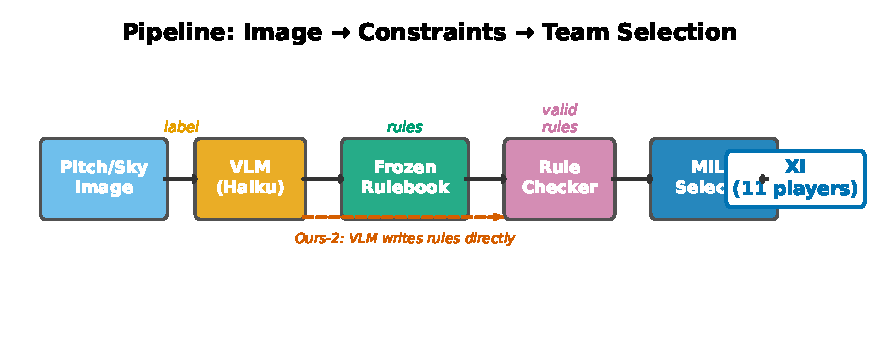
\includegraphics[width=\linewidth]{figures/fig1_pipeline.pdf}
\caption{Pipeline: a condition image (or weather text) $\to$ VLM (label or rules) $\to$ rulebook +
checker $\to$ MILP $\to$ XI $\to$ simulator $\to$ evaluation.}\label{fig:pipeline}
\end{figure}

\paragraph{Data and no-leakage.} We parse all men's T20Is from Cricsheet into tidy tables (matches,
XIs, deliveries), flagging super overs and rain/D-L games. Every feature, player value, venue prior
and simulator rate is computed only from matches strictly \emph{before} the match being evaluated, via
a single \texttt{history\_before} gate; a unit test fails if any feature reads a match on or after the
target date. Player bowling type (pace/spin) comes from the \texttt{cricketdata} \texttt{player\_meta}
table (no scraping).

\paragraph{Selection.} For each team--match we form a pool from the team's previous ten XIs (pool
coverage of the real XI is 90\%). A player's value is runs above average plus runs saved, with
empirical-Bayes shrinkage. A MILP (PuLP+HiGHS) picks exactly eleven players---at least one keeper and
five bowling options---maximising total value, subject to optional environment rules
$\mathrm{lo}\le\sum_{i\in\text{type}}x_i\le\mathrm{hi}$. Every selected XI's legality and value are
recomputed independently from player ids.

\paragraph{Conditions and rules.} A frozen rulebook maps condition labels to pace/spin bounds (e.g.\
dry $\Rightarrow n_\text{spin}\ge2$; green $\Rightarrow n_\text{pace}\ge3,\,n_\text{spin}\le1$). The
checker validates the schema, combines rule sets by the tighter bound with a fixed clash priority, and
relaxes any rule the pool cannot meet (logged). The VLM client (one interface over hosted and local
models, with strict JSON and $k$ runs) operates in a \emph{label} mode (mapped through the rulebook)
or a \emph{rules} mode (constraints written directly).

\paragraph{Simulator.} A vectorised ball-by-ball Monte Carlo draws each ball from a categorical
outcome distribution combining phase-shrunk batter and bowler rates; a \emph{condition-aware} variant
multiplies per-venue pace/spin wicket and boundary rates (fitted on an earlier window), and a
\emph{planted} variant injects known effects for synthetic scenarios. We use common random numbers
across arms and $\ge$10{,}000 sims per match.

\section{Experiments}
\paragraph{Arms.} B2 value-only; B3 cricket rules only; B4 oracle (true) environment rules; B5
venue-prior rules; B7 noisy rules (shift $\pm1$, pace/spin swap); Habit (team's usual spin count);
Ours-1 (VLM label$\to$rulebook); Ours-2 (VLM rules); Ref (real XI). Set R is \SetRN{} decisive
full-length 2025--26 matches between teams with $\ge$10 prior matches. Set S is a synthetic image set
with known pitch classes. The unit of analysis is the team--match; we report paired bootstrap 95\%
CIs (resampled by match), a Wilcoxon signed-rank test for $\Delta P(\text{win})$, and Holm correction
over the pre-registered arm comparisons.

\paragraph{Simulator validation.} On held-out matches the blind simulator attains Brier
\SimBlindBrier{} and AUC \SimBlindAUC{} ($n=\SimNMatches$), beating the coin-flip references
(0.25/0.5); the condition-aware simulator is within Monte-Carlo noise (Brier \SimCABrier, AUC
\SimCAAUC). The venue effect is near-symmetric across the two teams, so it barely changes win
\emph{prediction}; its role is to make the \emph{decision} sensitive to pace/spin balance.

\section{Results}
\begin{figure}[t]\centering
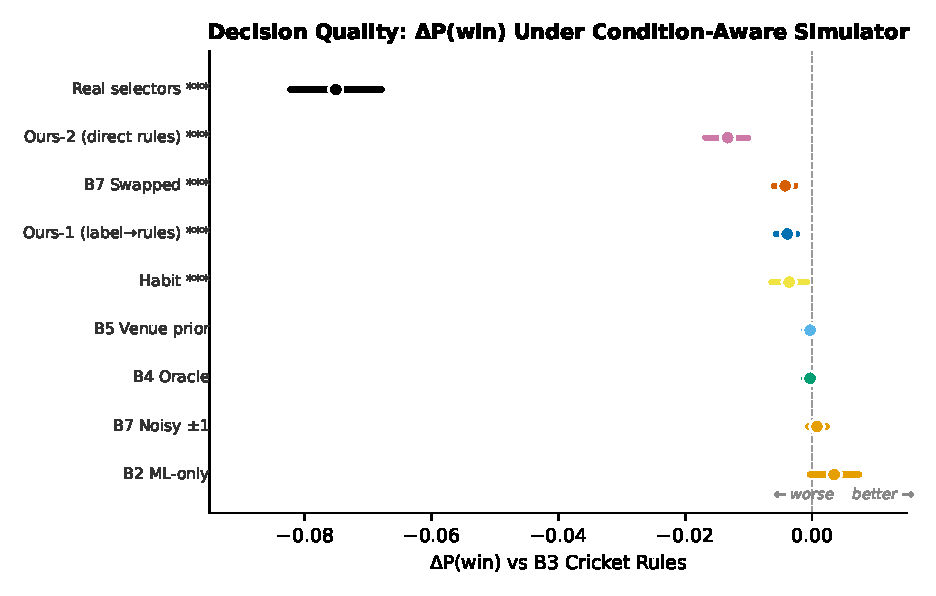
\includegraphics[width=\linewidth]{figures/fig4_delta_pwin.pdf}
\caption{$\Delta P(\text{win})$ vs.\ B3 by arm on Set R (95\% CI), under the blind and condition-aware
simulators. Correct rules (B4/B5) sit at zero; wrong rules (swap, Habit) are negative.}\label{fig:delta}
\end{figure}

\paragraph{Correct rules rarely change the decision.} The oracle/venue-prior rule changes the XI only
\OracleChange\% of the time and moves win probability by $\OracleDelta$ (95\% CI
$[\OracleCIlo,\OracleCIhi]$)---indistinguishable from zero---because the value-maximising baseline
already selects a balanced attack. Under the blind control the same arm gives $\OracleDeltaBlind$.

\paragraph{Wrong rules reliably hurt.} Swapping pace for spin gives $\SwapDelta$ (Holm $p=\SwapHolmP$)
and the ``habit'' rule $\HabitDelta$; the real selectors' XI is far from value-optimal under the
simulator ($\RefDelta$), as expected for a simulator that rewards our value proxy. This asymmetry
(zero for right, negative for wrong) shows the simulator is directionally sensitive while the decision
margin for \emph{adding} a correct constraint is small.

\begin{figure}[t]\centering
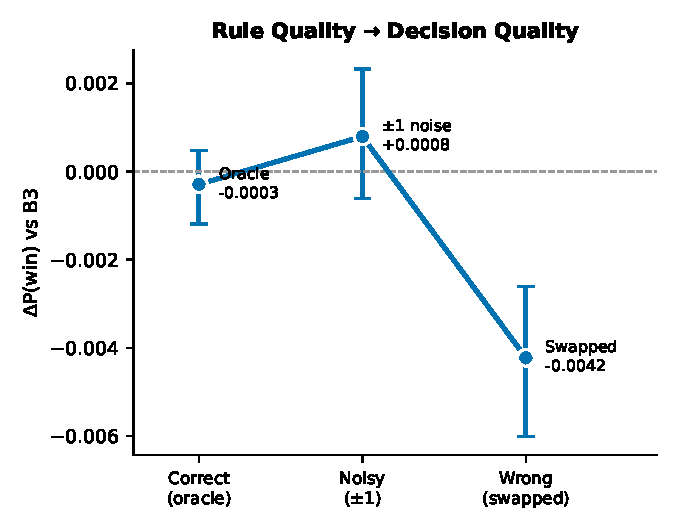
\includegraphics[width=\linewidth]{figures/fig6_noisy_rule.pdf}
\caption{Sensitivity to noisy rules (B7): as rules are perturbed (bound shifts, pace/spin swap), the
change in $P(\text{win})$ falls below that of correct rules.}\label{fig:noisy}
\end{figure}

\paragraph{Where the cost of wrong rules comes from.} The condition-aware simulator \emph{matched} the
blind one on held-out prediction (Brier \SimCABrier{} vs \SimBlindBrier, AUC \SimCAAUC{} vs
\SimBlindAUC, within Monte-Carlo noise), because the fitted venue pace/spin effect is near-symmetric
across the two teams. We state this plainly: the negative $\Delta P(\text{win})$ of wrong rules is
therefore \emph{entirely} the player value a mis-balanced XI gives up under the value model, not a
penalty from any modelled pitch effect. Our simulator does not reward getting the pace/spin mix
``right'' beyond its value consequences, so these results bound the decision value of \emph{correct}
constraints from below and should be read as a value-sacrifice accounting, not evidence that pitch
conditions change match outcomes.

\paragraph{Extraction quality.} On Set S the label mode is accurate---schema validity
\ExLabelSchema, exact set match \ExLabelExact, constraint F1 \ExLabelF, NL4Opt accuracy \ExLabelNL,
$k$-run Fleiss $\kappa=\ExLabelKappa$---while writing rules directly is noisier (exact \ExRulesExact,
F1 \ExRulesF). Under a planted simulator where conditions genuinely matter ($\pm$15\% effects,
\SetSCarriers{} carriers), even oracle constraints do not beat B3 ($\SetSPlantedOracle$): the player
value sacrificed by deviating outweighs the condition benefit at realistic effect sizes. Here the VLM
reader is \ReaderMain{}, reading real condition photographs synthesised locally with SDXL-Turbo (a
different model family from the readers, per our generation control); decoding is near-deterministic
so the reported $k$-run Fleiss $\kappa$ is high by construction.

\begin{figure}[t]\centering
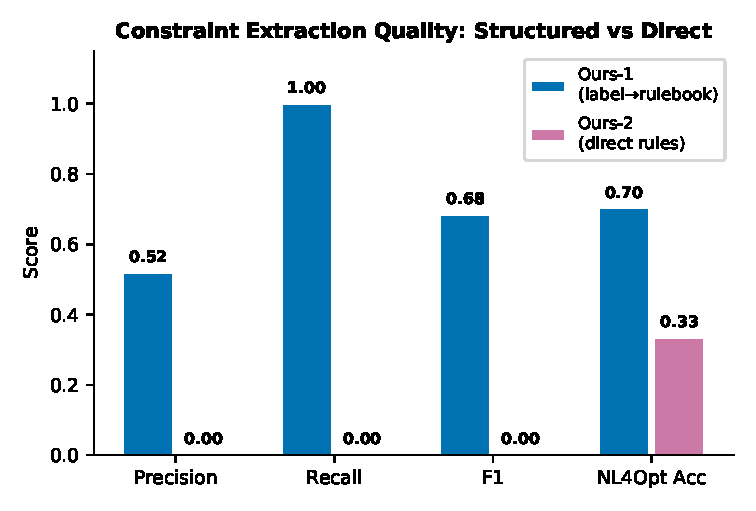
\includegraphics[width=\linewidth]{figures/fig3_extraction_f1.pdf}
\caption{Constraint-extraction F1 on Set S for label mode and rules mode.}\label{fig:f1}
\end{figure}

\paragraph{A second, small reader: per-class results.} The second VLM reader is Qwen3-VL:8b (8B
parameters, run locally via Ollama). Its overall label accuracy on Set S is 52\% (26/50) with schema
validity of 98\% (49/50 valid JSON). Per class (Figures~\ref{fig:perclass} and~\ref{fig:setsclass}),
it is perfect (100\%) on \emph{green}, \emph{dry}, \emph{wet} and \emph{uninformative}, partial (50\%)
on \emph{slow}, and fails (0\%) on \emph{clear}, \emph{overcast}, \emph{night}, \emph{rain\_now} and
\emph{flat}. Pitch-surface classes are thus easy even for a small VLM, whereas sky and weather classes
are hard, plausibly because SDXL-Turbo synthetic images lack realistic sky gradients; we have not
tested this explanation directly.

\begin{figure}[t]\centering
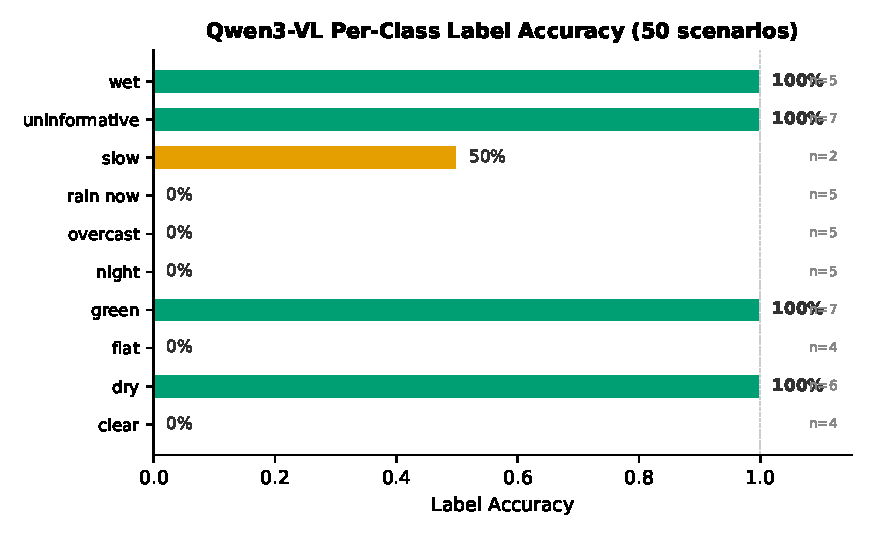
\includegraphics[width=\linewidth]{figures/fig2_per_class.pdf}
\caption{Qwen3-VL:8b per-class label accuracy on Set S.}\label{fig:perclass}
\end{figure}

\begin{figure}[t]\centering
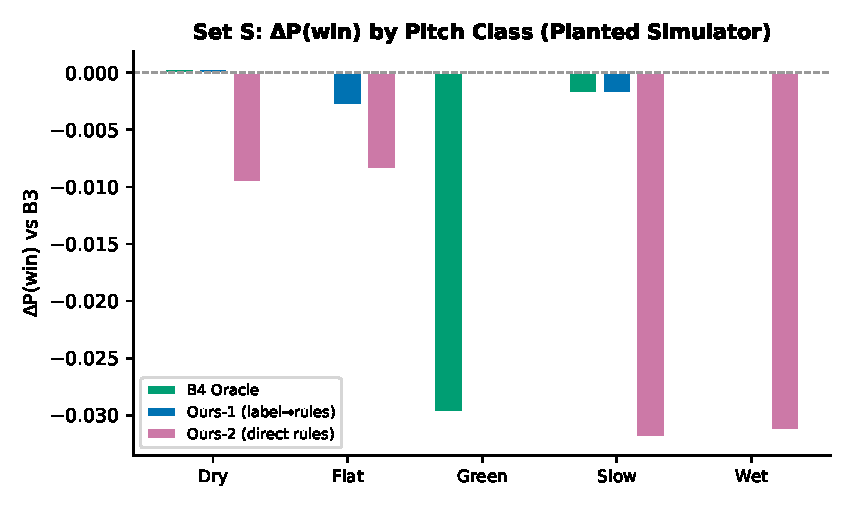
\includegraphics[width=\linewidth]{figures/fig5_set_s_class.pdf}
\caption{Set S results broken down by pitch class.}\label{fig:setsclass}
\end{figure}

\section{Limitations}
Results are simulator-based and exploratory; we make no claim of winning real matches. The
VLM-extraction figures are produced by \ReaderMain{} as the main reader, with a local open-weight
reader as a second family; under the current hosted API sampling parameters are rejected, so hosted
decoding is near-deterministic and $k$-run consistency is high by construction rather than estimated
under temperature. Synthetic condition images are generated \emph{locally} with SDXL-Turbo rather
than with Gemini as originally intended: the available Gemini key is free-tier and returns a hard
``\texttt{limit: 0}'' for every image model, so Gemini generation awaits a billed key (the code path
ships). The automated image check uses a CLIP zero-shot rater; a human rater check is still pending
before camera-ready. Bowling-type coverage is 78\% of bowlers (associate-nation players dominate the
remainder). The decision effect we measure is specific to our value objective and simulator; a
different objective or larger condition effects could change the sign.

\section{Data statement}
Match data: Cricsheet (\url{https://cricsheet.org}), ODC-By 1.0. Weather: Open-Meteo
(\url{https://open-meteo.com}), CC BY 4.0. Player metadata: the \texttt{cricketdata} R package
(rOpenSci). Synthetic images generated by us. No scraping of ESPNcricinfo, Cricbuzz or Getty. Code and
every number are reproducible from cache via \texttt{scripts/run\_vision\_constraints.py --all}.

\bibliographystyle{plain}
\bibliography{refs}
\end{document}
